\documentclass{article}
\usepackage[margin=0pt,paperwidth=8cm,paperheight=13cm]{geometry}
\usepackage{tikz}
\usetikzlibrary{shapes.geometric, arrows, positioning, fit}
\begin{document}
\thispagestyle{empty}
\vspace*{2pt}
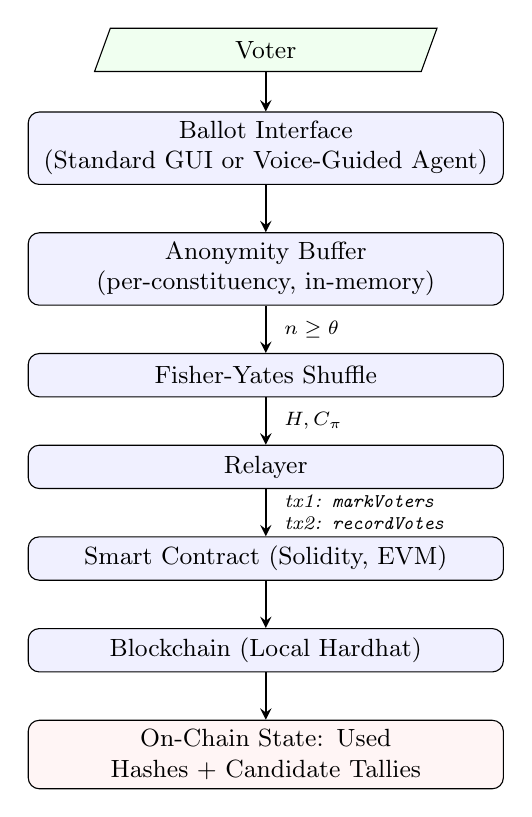
\begin{tikzpicture}[
  node distance=0.6cm,
  box/.style={rectangle, draw, fill=blue!6, rounded corners, text width=5.8cm, align=center, minimum height=0.55cm, font=\small},
  io/.style={trapezium, trapezium left angle=70, trapezium right angle=110, draw, fill=green!6, text width=3cm, align=center, minimum height=0.55cm, font=\small},
  arrow/.style={->, thick, >=stealth},
  label/.style={font=\scriptsize\itshape},
  dashedbox/.style={rectangle, dashed, draw=blue!50, rounded corners, inner sep=4pt}
]
  \node[io] (voter) {Voter};

  \node[box, below=0.5cm of voter] (ui) {Ballot Interface\\\small(Standard GUI or Voice-Guided Agent)};

  \node[box, below=of ui] (buffer) {Anonymity Buffer\\\small(per-constituency, in-memory)};

  \node[box, below=of buffer] (shuffle) {Fisher-Yates Shuffle};

  \node[box, below=of shuffle] (relayer) {Relayer};

  \node[box, below=of relayer] (contract) {Smart Contract (Solidity, EVM)};

  \node[box, below=of contract] (chain) {Blockchain (Local Hardhat)};

  \node[box, below=of chain, fill=red!4] (data) {On-Chain State: Used Hashes + Candidate Tallies};

  \draw[arrow] (voter.south) -- (ui.north);
  \draw[arrow] (ui.south) -- (buffer.north);
  \draw[arrow] (buffer.south) -- (shuffle.north) node[midway, right, label] {\ $n \geq \theta$};
  \draw[arrow] (shuffle.south) -- (relayer.north) node[midway, right, label] {\ $H, C_\pi$};
  \draw[arrow] (relayer.south) -- (contract.north)
    node[midway, right, label, align=left] {\ tx1: \texttt{markVoters}\\ \ tx2: \texttt{recordVotes}};
  \draw[arrow] (contract.south) -- (chain.north);
  \draw[arrow] (chain.south) -- (data.north);
\end{tikzpicture}
\vfill
\end{document}
